\documentclass[landscape,paperwidth=43truein,paperheight=33.1truein,fontscale=0.3]{baposter}
\usepackage{graphics}
\usepackage{color}
\usepackage{multicol}
\usepackage{amsmath}
\usepackage{amssymb, wasysym}
\usepackage{lipsum}
\usepackage{graphicx}
\usepackage{enumitem}

\pdfcompresslevel=1

\begin{document}
\definecolor{myfavoritecolor}{rgb}{0.0 2.55 0}

%:Background image
\background{
      \begin{tikzpicture}[remember picture,overlay]%
      \draw (current page.center)+(-0em,-10em) node[anchor=center]
      {\includegraphics[width=1.2\textwidth]{images/blue_sun}};
      \end{tikzpicture}%
      }

\begin{poster}
{%Keyword=value pairs
  % Color style
background = user,
 bgColorOne=white,
  bgColorTwo=red,
  borderColor=black,
  headerColorOne=black,
  headerColorTwo=gray,
  headerFontColor=white,
  boxColorOne=white,
  boxColorTwo=myfavoritecolor,
  % Format of textbox
  textborder=roundedleft,
  % Format of text header
  eyecatcher=true,
  headerborder=closed,
  headerheight=0.15\textheight,
  headershape=roundedright,
  headershade=shadelr,
  boxshade=plain,
  headerfont=\Large\textrm,
}
{%Eyecatcher
   \resizebox{!}{.18\textheight}{
\includegraphics{images/inverted_solar_physics_logo.png}}
}
{%Poster Title
   {\color{red}Software Development for MOSES Flight Operations}
}
{%Author
  \color{red} \textbf{Roy Smart, Jackson Remington, David Keltgen, Justin Hogan, Charles C.\ Kankelborg\\
   \textit{Physics Department, Montana State University, Bozeman, MT 59717}\\
   roytsmart@gmail.com}\\
}
{%Logo
   \resizebox{!}{.13\textheight}{
\includegraphics{images/msuvertcmyk.pdf}}
}

%%%%%%%%%%%%%%%%%%%%%%%%%%%%%%%%%%%%
%         Zeroth Column            %
%%%%%%%%%%%%%%%%%%%%%%%%%%%%%%%%%%%%

\headerbox{Abstract}{name=abstract,column=0}{
 The Multi Order Solar EUV Spectrograph (MOSES) sounding rocket payload is a slitless spectrograph that allows snapshot imaging spectroscopy of the Sun in extreme ultraviolet (EUV) wavelengths
$^{[0]}$. The MOSES payload relies on an embedded flight computer and FPGA
to control the instrument, command exposures from the cameras, save the experimental data, and send
the data with additional telemetry back to Earth. Replacing the previous command and data handling
system with a low-power solution necessitated the development of new software that could satisfy the
same requirements as last mission while improving on the latencies present in the old flight software. 
The new configuration is still in development, and is undergoing debugging and optimization in preparation for launch. \vspace{0.33cm}
}

\headerbox{First Launch}{name=launch,column=1}{
\begin{tabular}{ll}
 \begin{minipage}{0.10\columnwidth}
      \resizebox{\columnwidth}{!}{\includegraphics{images/MOSESinFlight.png}}
   \end{minipage} &
   \begin{minipage}{0.80\columnwidth}
      \textit{MOSES} was 
      first launched on February 8, 2006 on a NASA sounding rocket. The next launch will include updated optics and electronics and is scheduled for summer 2015.
   \end{minipage} 
  
\end{tabular}
}

\headerbox{Design Challenges}{name=challenges,column=2}{
	The sounding rocket trajectory only provides approximately 5 minutes of data for the instrument to capture. To acquire data in real time and minimize risk to the experiment, the flight software must be efficient and use minimal resources. \vspace{.21cm}
}

\headerbox{Data Interface}{name=interface,column=1,span=2, below=launch}{

\begin{tabular}{ll}
  \begin{minipage}{0.50\columnwidth}
The new flight computer is designed as a drop-in replacement for the old flight computer, so it must interface with the instrument in the same manner. The primary means of starting and stopping the experiment are predefined \textbf{Timers}. Science data is acquired from the \textbf{ROE} using the \textbf{FPGA}. It is then transferred to the \textbf{VDX} using DMA and written to disk. For redundancy, the data is transmitted to earth using the \textbf{Synclink USB} interface and a 10 Mbit/s link.

  \end{minipage}&
  \begin{minipage}{0.45\columnwidth}
      \resizebox{\columnwidth}{!}{\includegraphics{images/hw_block}}
      \footnotesize{Block diagram of major hardware components managed by flight software}  
\end{minipage}  
\end{tabular}


}
\headerbox{Hardware Solutions}{name=hardware,column=3}{
The VDX104+ running a Ubuntu GNU/Linux operating system is the flight computer for the instrument. It provides ethernet and RS-232 serial ports for communication, and PCI-104 bus for interfacing with the FPGA. The flight software designed by our team runs on this device.

\begin{tabular}{ll}
	\begin{minipage}{0.46\columnwidth}
  		\resizebox{\columnwidth}{!}{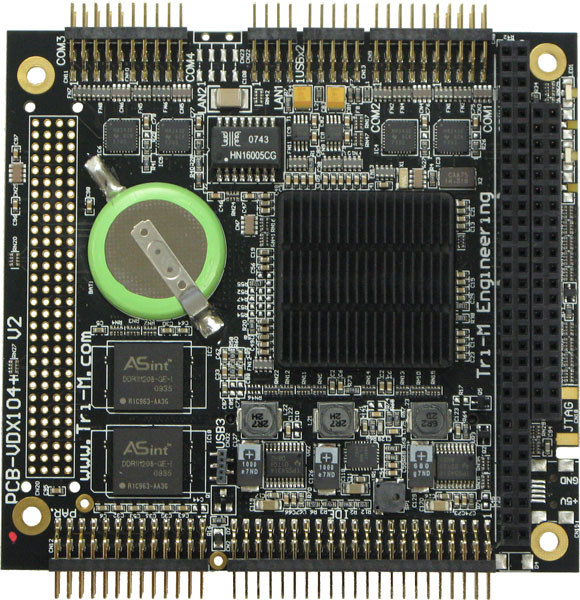
\includegraphics{images/vdx104}}  \\
  		\footnotesize{VDX104 flight computer}
	\end{minipage}&

  \begin{minipage}{0.46\columnwidth}
		\resizebox{\columnwidth}{!}{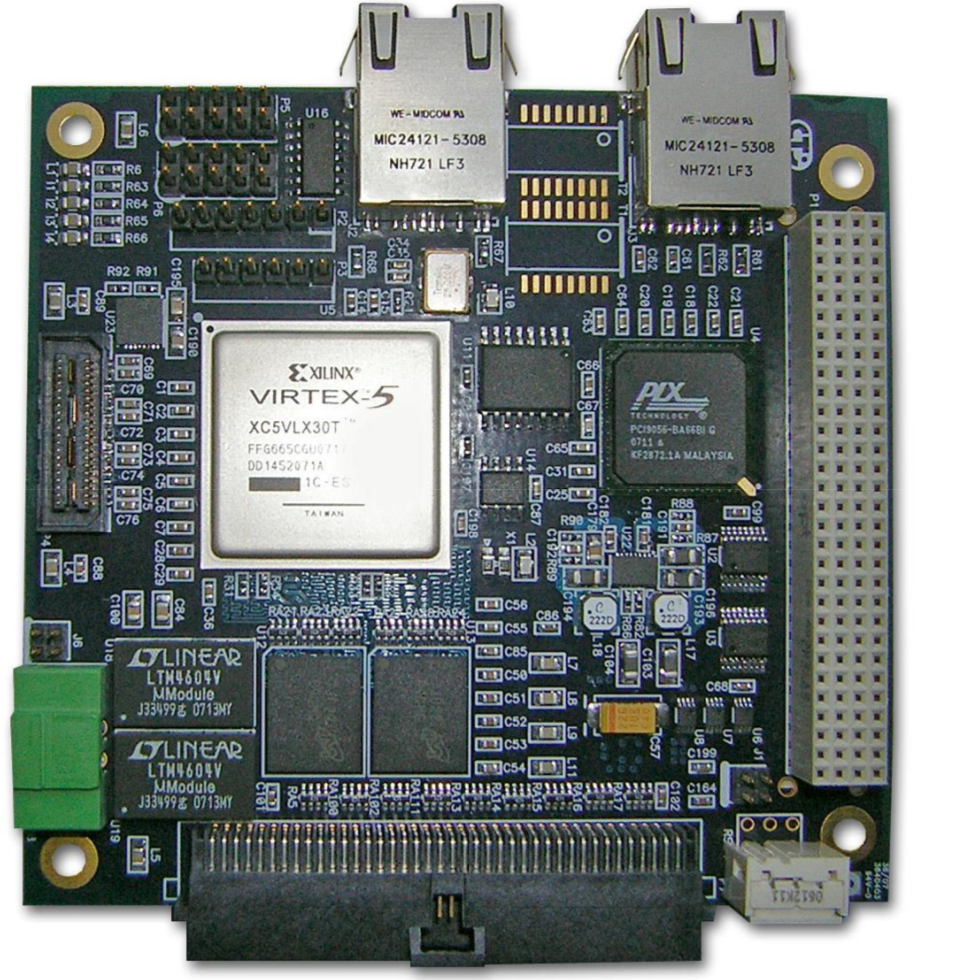
\includegraphics{images/fpga}} \\
		\footnotesize{ Virtex5 FPGA}
  \end{minipage}
\end{tabular} \\ \\
The Virtex5 FPGA captures the 32 Mbit/s parallel data produced by the experiment and various GPIO. It then transfers the data through DMA to the flight computer for processing.

}

\headerbox{Software Architecture}{name=arch,column=0,span=3, below=interface}{
\begin{tabular}{ll}
	\begin{minipage}{0.85\columnwidth}
      \resizebox{\columnwidth}{!}{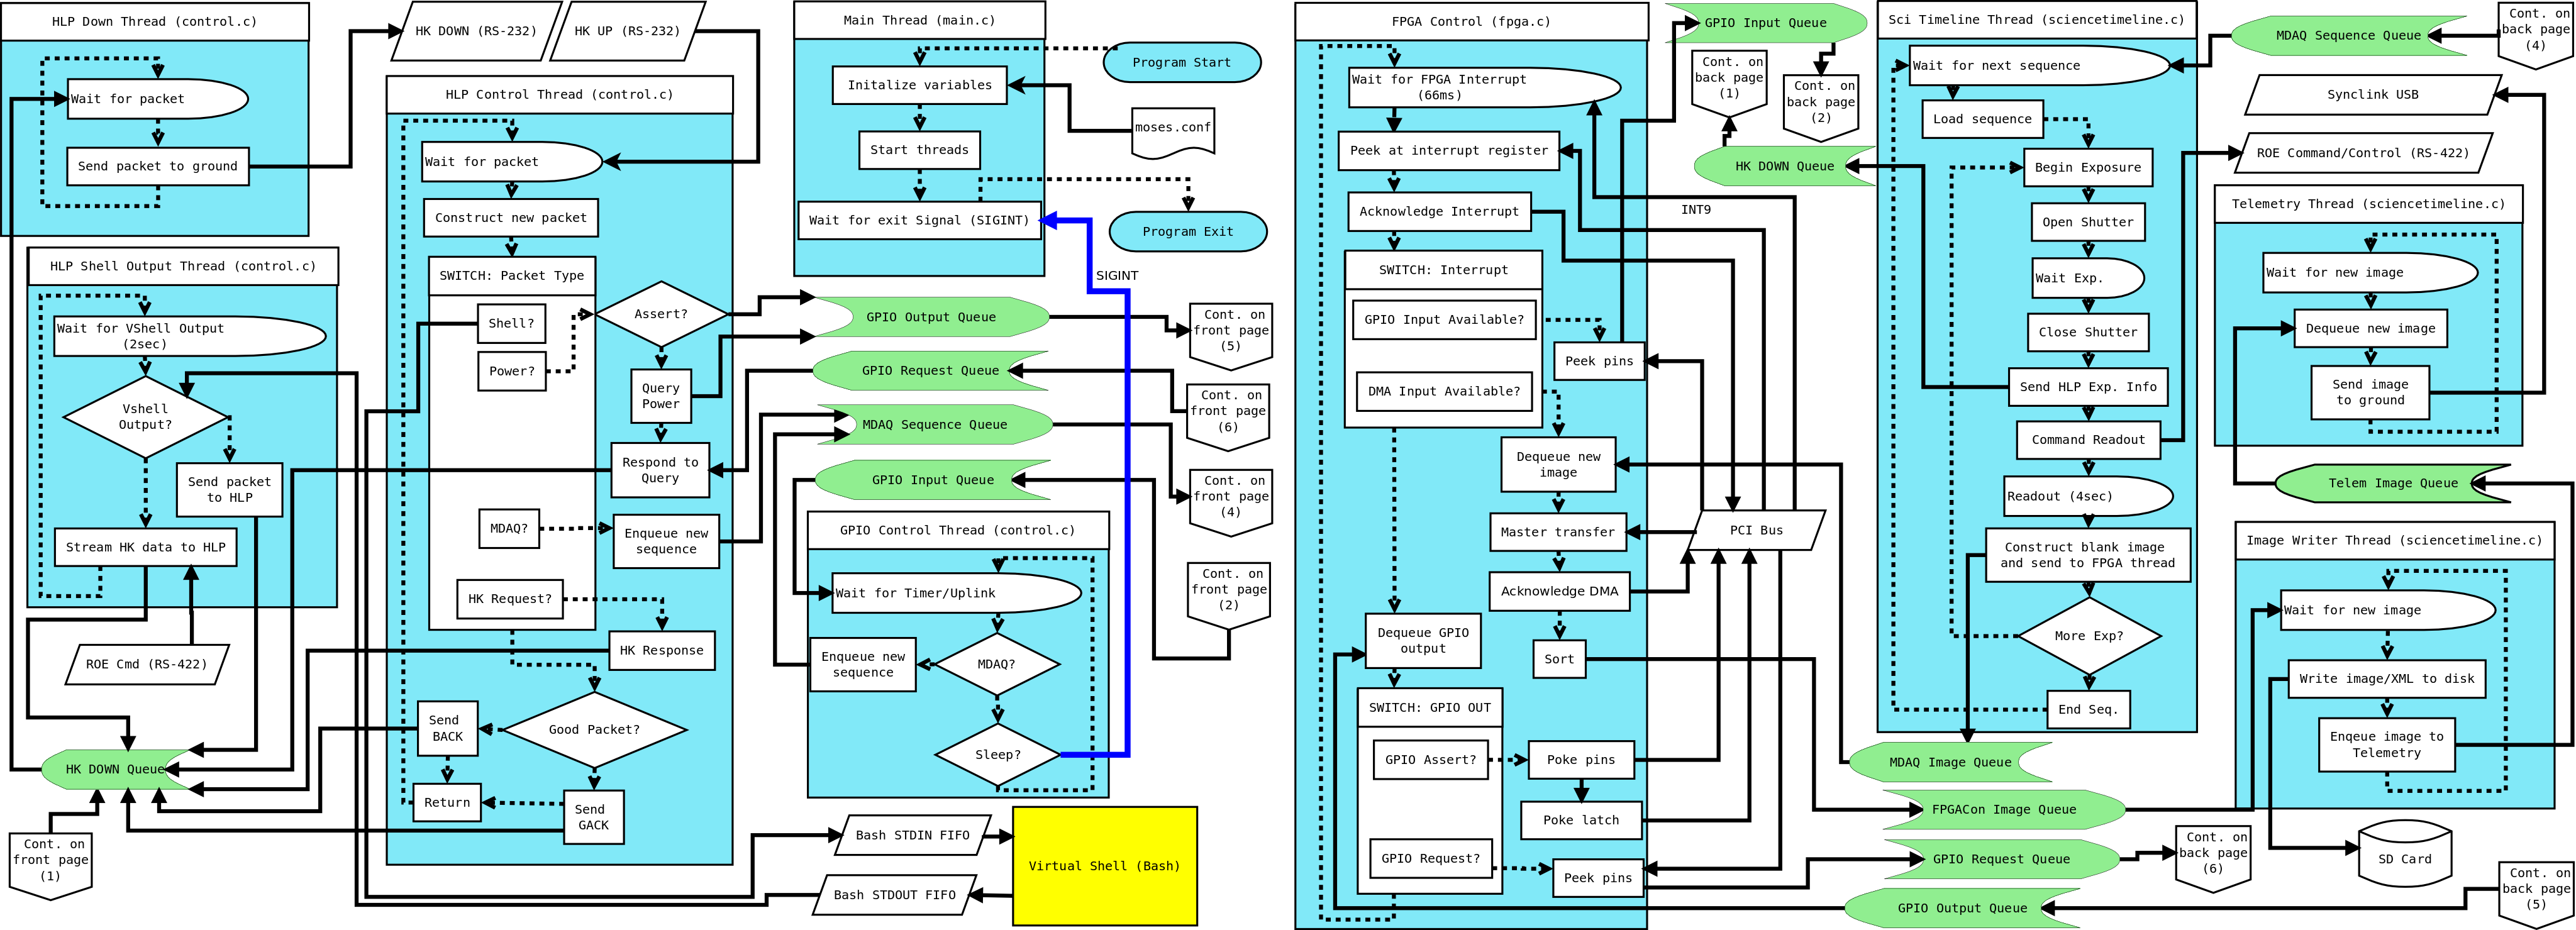
\includegraphics{images/mfsw_block}}
      \footnotesize{Diagram of major software modules}  
	\end{minipage}&

  \begin{minipage}{0.10\columnwidth}
  	\raggedright
     The flight software relies on a threaded architecture to reliably respond to a variety of inputs, all while the processor is actively capturing data. Several thread-synchronization techniques have been utilized, including mutex-protected queues, Linux Signals, and semaphores. 

  \end{minipage}
    
\end{tabular}
}

\headerbox{Glossary}{name=gloss,column=3,below=hardware}{ 

%\begin{itemize} \itemsep1pt \parskip0pt \parsep0pt \itemindent=-0.5cm
\begin{itemize}[leftmargin=*, noitemsep]
\item \textbf{EUV:} Extreme Ultraviolet electromagnetic radiation.
\item \textbf{VDX:} Model name of flight computer board.
\item \textbf{FPGA:} Field-Programmable Gate Array. 
\item \textbf{ROE:} Read-Out Electronics. Hardware that captures science data from cameras.
\item \textbf{DMA:} Direct Memory Access. Protocol for copying data without involving the computer's processor.
\item \textbf{HLP:} Housekeeping Link Protocol. Packets transmitted from the ground that can control the instrument.
\end{itemize}
}


\headerbox{Acknowledgment}{name=ack,column=3,below=gloss}{ \footnotesize

\begin{minipage}{\columnwidth}
This work is supported by the NASA Sounding Rocket Program, Grant NNX14AK71G.
 
\end{minipage}
\normalsize
}


\headerbox{References}{name=refs,column=3,below=ack,above=bottom}{\footnotesize
\begin{minipage}{\columnwidth}
[0] Fox, Kankelborg and Thomas, 2010 \textit{Astrophys.J.}, 719:1132-1143

[1] Background image courtesy of the NASA Solar Dynamics Observatory
 
\end{minipage}
\normalsize}

\end{poster}

\end{document}